\section{Methodology}

As revealed in the literature review, there is a gap in a general-purpose
networking framework in smartphone-based ad hoc networking. The existing
implementation of the framework partially fills the gap. However, the current
framework only uses Bluetooth Classic and Bluetooth Low-Energy technologies to
communicate. This can be improved by using Wi-Fi Direct technology. Moreover,
the routing algorithm used in the current framework can be further enhanced
after research on the performance of routing algorithms. In the following
sections, the core technologies used will be discussed.

\subsection{Modular Framework}

Our objective is to enhance the existing implementation by introducing a
modularized framework while also striving to incorporate WiFi Direct
functionality. This improved framework will continue to serve as a versatile
platform for sharing text messages among network nodes and will subsequently be
extended to facilitate seamless media and file transfers.

The previous implementation was primarily centered around Bluetooth Classic and
BLE technologies, allowing us to address a specific range of communication
needs. In this upgraded version, we aim to diversify the connectivity options
by exploring the capabilities of WiFi Direct. This will enable us to harness
the benefits of high-speed communication over Wi-Fi connections, complementing
the existing Bluetooth functionalities.

By modularizing the framework, we intend to enhance its flexibility and
scalability, making it easier to customize and adapt to different applications
and use cases. This approach will facilitate the integration of new Transport
modes other than the ones mentioned.

The following figure~\ref{figArch} shows a high-level diagram of the upgraded
framework. A brief description of the components is given below.

\begin{itemize}
    \item \textbf{MeshifyClient:} This behaves as an entry point for
          application programmers.
    \item \textbf{DiscoveryManager:} Used in the neighbor discovery process
          using the implemented neighbor discovery protocol
    \item \textbf{ConnectionManager:} Manages device connections
    \item \textbf{FowardController:} Manages message passing in multihop
          communication
    \item \textbf{TransportManage:} Manages the communication between the
          Android layer and the framework based on the Transports in a modular
          way.
\end{itemize}

\begin{figure}[htbp]
    \centerline{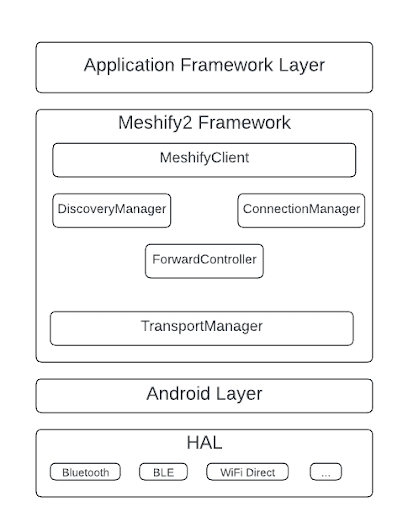
\includegraphics[height=0.45\textwidth]{imgs/classArch.png}}
    \caption{Upgraded Framework}
    \label{figArch}
\end{figure}

\subsection{Bluetooth and Bluetooth Low Energy}

\subsubsection{Bluetooth Classic}

In classic Bluetooth, an inquiry device transmits inquiry packets called
identification packets(ID packets) and listens to inquiry responses called FHS
(Frequency Hop Synchronization) packets. The neighboring devices must be in an
inquiry scan to receive ID packets and reply with FHS packets. ID packets give
no information about the inquiry device. But FHS packets have the Bluetooth
address and other information about the responding device. Also, the inquiry
process does not establish any connection. Connection is established in the
page procedure where a device responds in its page scan procedure to the device
that carries out the paging. This paging is only targeted for a single device
identified in the inquiry process. The paging device is considered the master
device for the connection. Responding devices are the slaves, and every device
can become a slave or a master, and the roles can be switched within a
connection. Piconet is the basic Bluetooth topology, which consists of a master
and slaves, and the active slaves for a master should be seven or fewer. A
Bluetooth scatternet consists of more than one piconet. As explained in
neighbor discovery protocols, they can be categorized as direct and indirect.
Only the immediate neighboring nodes are discovered in the direct method, and
in the indirect method, nodes can learn about other existing nodes through
their neighboring nodes\cite{todtenberg2019}.

In the Meshify Framework, a Bluetooth device can act as both a client and a
master, and each role has its thread to do so\cite{gunasekara2022}. One thread
is set as discoverable for incoming connections, while the other thread
performs scanning. Also, the Bluetooth discovery protocol allows the devices to
be connected without pairing.

\begin{figure}[htbp]
    \centerline{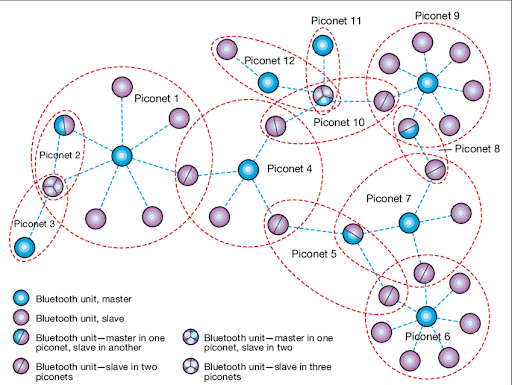
\includegraphics[height=0.45\textwidth]{imgs/piconetbl.png}}
    \caption{Bluetooth Scatternet Diagram consisting of several piconets
        \cite{Larsson2000}}
    \label{piconetbl}
\end{figure}

\subsubsection{Bluetooth Low Energy}

‘Scanners ’ listen for advertising events actively broadcasted by ‘Advertisers’
over the physical channels. Since the scanners can initiate a connection after
receiving from an Advertiser, they are also called “Initiators.” After the
advertiser accepts the connection request, the scanning device becomes the
master, and the advertising device becomes the slave. Also, the BLE
specifications don't limit the number of slaves. In Piconet, they don’t use a
shared frequency channel, and the master gives a unique hopping sequence
point-to-point for each slave. So the master uses the polling technique to
communicate with its slaves consecutively using time division multiplexing
\cite{todtenberg2019}.

\begin{figure}[htbp]
    \centerline{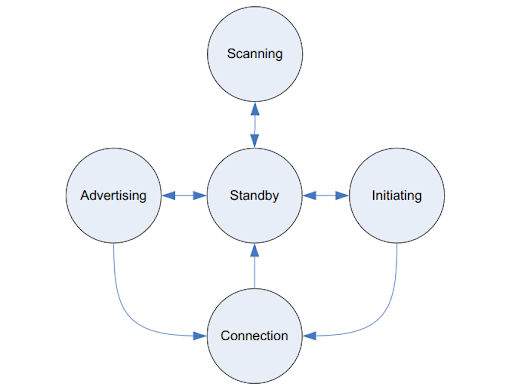
\includegraphics[height=0.45\textwidth]{imgs/blstatemach.png}}
    \caption{BLE State Machine}
    \label{blstatemach}
\end{figure}

\subsubsection{Neighbor Discovery Process for Meshify}

When a client connects with the master, the client sends a handshake packet
containing its Meshify UUID. Master adds the client to its neighbor devices
list and sends the handshake ack containing its UUID and the neighbor list. So,
the client adds the master and the neighbor list to its neighbor list. Since
when a client sets a connection with the master, all the other clients should
know about the new client, the master responds with a
broadcast\cite{gunasekara2022}.

\begin{figure}[htbp]
    \centerline{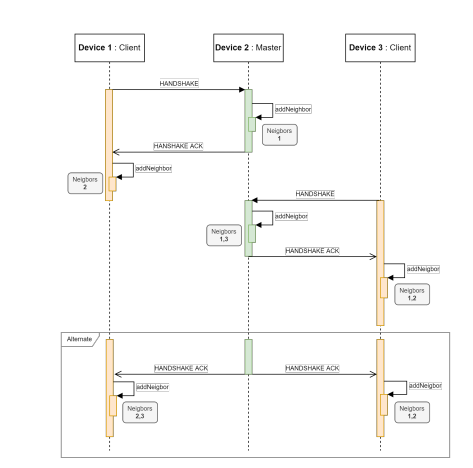
\includegraphics[height=0.75\textwidth]{imgs/neighbourdis.png}}
    \caption{Neighbour Discovery Process for Meshify\cite{gunasekara2022}}
    \label{neighbourdis}
\end{figure}

\subsubsection{Routing for Meshify}

Meshify utilizes TARP, a simple routing protocol, to route traffic via a
controlled flooding method. TARP is a layer-less routing scheme that was
created for Wireless Sensor Networks. The protocol is a set of rules a node
must follow to process each packet\cite{gunasekara2022}. According to
\cite{wsn2021} in TARP, unless there is a specific reason not to do so, a node
floods the packet to all surrounding nodes.

\begin{figure}[htbp]
    \centerline{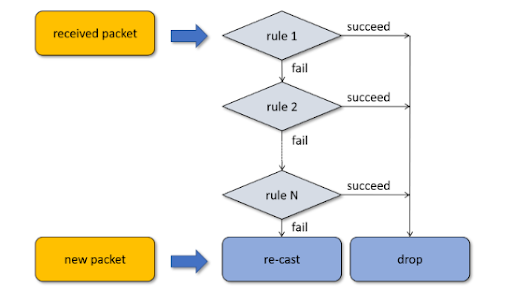
\includegraphics[height=0.45\textwidth]{imgs/tarpproc.png}}
    \caption{The mechanism of TARP \cite{wsn2021}}
    \label{tarpproc}
\end{figure}

As seen in Fig.~\ref{tarpproc}, the rules will be implemented in the order
listed, beginning with rule number 1 and progressing to the last rule. If a
specified rule is met, the packet is dropped. Following a rule implies
determining a reason to drop the packet. A rule can examine the full packet of
data being transmitted and use any criteria it desires to determine what to do
with that data. This rule can receive the packet, change what's inside, or
generate a new delivery packet. Some rules have specific expectations about
what is in the packet, and the application employing these rules can adapt them
to meet its particular requirements\cite{wsn2021}.

Gburzyński\cite{wsn2021} discusses some main rules used in TARP.

\begin{itemize}
    \item Limit Hop Count (LHC) - This rule restricts the number of hops a
          packet can take. Following the creation of a packet by a source, the
          number of
          forwardings to which the packet was subjected is counted, including
          the initial
          transmission. When the number of hops for a specific packet reaches
          the
          maximum, the packet is dropped.

    \item Duplicate Discard (DD) - This rule attempts to prevent the same
          packet from being sent numerous times. Each packet contains a unique
          identifier
          known as a serial number. When a node forwards a packet, it stores a
          signature
          that is a combination of the sender's address and the packet's serial
          number.
          If the node already possesses the signature, the packet will be
          dropped because
          it has previously been delivered through this node.

    \item Sub-optimal Path Discard (SPD) - Using the rule DD, a node listens to
          another node delivering a packet and determines the shortest number
          of hops to
          reach that node. Assume an intermediary node exists between the
          sender and
          destination nodes. The intermediate node has the fewest hops from the
          sender to
          that node and from that node to the destination. If the sum of the
          hops is
          larger than the smallest number of hops from the sender to the
          destination
          node, the packet will bypass the intermediate node.

\end{itemize}

All of the TARP rules outlined above govern the flooding process for Meshify.
Aside from the TARP restrictions, the Meshify has single-hop acknowledgments to
improve reliability. However, because this can reduce throughput, only the
packet's destination sends single-hop acknowledgments to its
neighbors\cite{gunasekara2022}.

\subsection{Wifi-Direct}

Wi-Fi Direct is a P2P communication standard complying with the IEEE 802.11
standard. The core purpose of the standard is to enable WiFi-enabled mobile
devices to connect to printers and other WiFi-enabled devices in a peer-to-peer
manner\cite{malar2023}.

Compared with the Bluetooth and Bluetooth Low Energy standards described above,
WiFi Direct as a communication method has two main advantages.

\begin{itemize}
    \item Speed: As Malar et al. present, WiFi connections have a speed greater
          than 54Mbit/s while Bluetooth speed is limited to 3 Mbit/s. This is
          advantageous in facilitating fast file transfer.

    \item Security: WiFi Direct uses the WPA2 standard, which is more secure
          for data transfers than Bluetooth.
          Therefore, implementing a multi-hop ad hoc network using WiFi Direct
          is
          advantageous.

\end{itemize}

\vspace{0.3cm}

\subsubsection{Operation of Wifi-Direct}
WiFi Direct (WiFiDi) is primarily a P2P standard operating in a functional
structure called a Group. A group consists of a Group Owner and a set of P2P
clients (referred to as a Group Member) that connect as peers to the Group
Owner. In WiFiDi, the roles of the devices, whether a P2P client or a Group
Owner (GO), are not predetermined but negotiated at group formation.

Only devices conforming to the standard are equipped to participate in the
group formation procedure. However, once the group is established, devices
without WiFiDi can connect to the GO as an ordinary WiFi
client\cite{funai2015}\cite{wifidispec}. This case can be referred to as a
Legacy Client.

\begin{figure}[htbp]
    \centerline{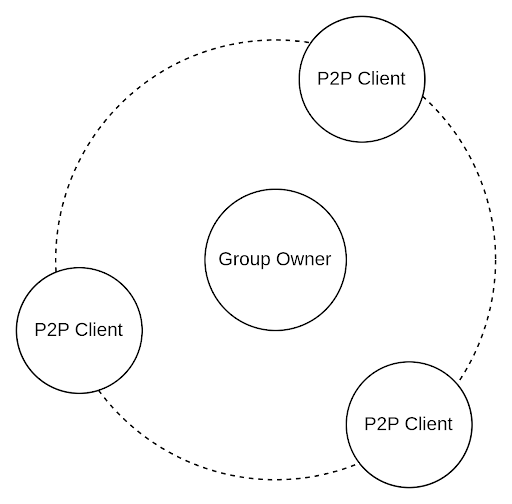
\includegraphics[height=0.45\textwidth]{imgs/group.png}}
    \caption{A WiFi-Direct Group}
    \label{digroup}
\end{figure}

\subsubsection{Group Formation Procedure}

Before the group formation begins, all devices not currently in a WiFiDi group
are put into a listen state where the devices listen in a given “listen
channel”; this channel is selected from the “social channels” set. In the
2.4Ghz band the list of social channels is 1, 6, and 11\cite{wifidispec}. Once
devices are discovered they move to the group formation phase.

There are two main stages of group formation and three main modes of group
formation the nodes can be configured to follow. The following section
describes the standard group formation action flow.

\begin{enumerate}
    \item Group owner negotiation

          Considering the case of two devices performing a negotiation, a
          handshake of three frames is implemented by the standard. Each frame
          contains
          the device information, P2P capabilities and owner
          intent\cite{wifidispec}.
          Owner intent is a metric of the device’s intent of becoming a group
          member. This process is outlined by Fig.~\ref{formproc}
          %add the thing here

    \item Provisioning

          The provisioning step sets up the group following the WiFi Protected
          Setup\cite{wifidispec}, allowing the group members to share data in
          secure
          sessions.

\end{enumerate}

\begin{figure}[htbp]
    \centerline{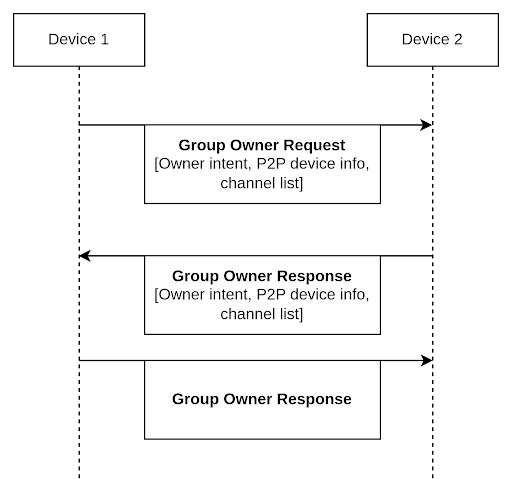
\includegraphics[height=0.45\textwidth]{imgs/formproc.png}}
    \caption{Standard WiFi Group Formation Procedure}
    \label{formproc}
\end{figure}

\subsubsection{Intra-Group Routing}

After the group owner is established and the group is provisioned, the group
owner acts as a DHCP host to provide IP addresses to each peer in the
group\cite{funai2015}. The group owner then acts as a Soft-Access Point and
controls routing between nodes within the group and other network operational
and management functions such as channel management\cite{wifidispec}.

\subsubsection{Inter-group routing (Multi-hop Routing)}

As mentioned above, the WiFiDi standard ensures P2P communication between the
Group Owner and the Group Members, and by the soft-AP role of the Group Owner,
the routing within the group. However, the standard does not provide any
mechanism for multi-hop routing.

However, there are two possible ways of achieving this. All two methods involve
a gateway node, either temporarily or permanently connected to more than one
group. The simultaneous connection of a single node to two different groups is
not excluded in the standard. However, the functionality of such an arrangement
may depend on the specific implementation of the standard\cite{funai2015}.

According to Funai et al., the gateway can be either a group member or legacy
client of either group and in the second scenario, the gateway node can also be
a group owner in one and a group member or a legacy client in the second
group\cite{funai2015}.

However, it is impossible to directly implement these strategies due to the
Android operating system limitations.

For example, as observed by Funai et al., when the gateway node is a group
member of one group and a legacy client of the other group, the gateway could
receive packets from both groups. Still, it could not send outgoing packets to
either\cite{funai2015}.

Funai et al.\cite{funai2015} presented two mechanisms to overcome this.

\begin{enumerate}
    \item A timeshare mechanism
          As presented in Fig~\ref{timeshare}, this mechanism, the gateway node
          can
          disconnect from the source group
          and dynamically connect to the destination group at packet transfer.
          The
          Android APIs do not supplement the switching process and must be
          handled at the
          application level\cite{funai2015}.
    \item Simultaneous connection
          Authors found that it is possible to use the gateway node as a group
          member
          in one group and a local client in the other to transfer data using
          the UDP
          multicast socket supplied in Android\cite{funai2015}.
\end{enumerate}

\begin{figure}[htbp]
    \centerline{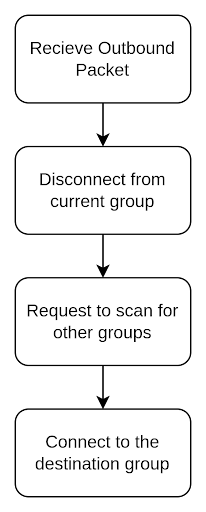
\includegraphics[height=0.45\textwidth]{imgs/timeshare.png}}
    \caption{Gateway Node Timeshare Procedure}
    \label{timeshare}
\end{figure}

\vspace{0.3cm}

\subsubsection{Android SDK and WiFi Direct}
The main WiFi Direct functionality in Android is provided by the WiFiP2pManager
class in the Android SDK. This class allows for the complete group creation and
other related operations in the WiFiDi standard.

Following are the core methods in WiFi Direct implementation\cite{wifiman}.

\begin{itemize}
    \item discoverPeers(): Discover available peers
    \item createGroup(): Initiate the group creation mechanism
    \item removeGroup(): Remove the currently connected group
    \item requestGroupInfo(): Request for the connected group info
\end{itemize}

\vspace{0.1cm}

This API can create an application layer framework capable of performing
inter-group(multi-hop) routing.

\subsection{Simulations and Testing}

It is vital to test the proposed framework and the applications during and
after the development process to ensure that the network traffic is handled
properly at different levels of traffic and mesh scenarios. Morote et al.
provide a mechanism for testing routing protocols with the open-source software
module called Network Simulator 2\cite{morote2010}. The newest version of
Network Simulator is version 3, commonly known as ns-3\cite{ns3}. Ns-3 is a
discrete event simulation platform written in C++ and it supports OTcl scripting
language for modeling node mobility\cite{morote2010}. However, our simulation
scenario is different from the standard testing scenario for ns-3 due to the
fact that the routing and other features are handled on the application layer.

Another simulation platform available is the OMNET++ simulation platform. The
platform allows simulating nodes and network event behaviors using C++ classes
and also provides an IDE and a graphical simulator runner\cite{opensim}. We aim to
use this platform to simulate the framework and test under different mobility
scenarios.

Therefore, we aim to simulate the framework on the ns3 platform and test under
different scenarios of node availability and mobility.

\vspace{0.3cm}

\subsubsection{Simulation Plan}
The existing simulations and results will be extended by adding the following
specifications and analyzing the results.

\vspace{0.3cm}

Comparative routing protocols:
\begin{itemize}
    \item TARP
    \item AODV
    \item DSDV
\end{itemize}

\vspace{0.3cm}

Mobility Models:
\begin{itemize}
    \item Gauss-Markov Mobility Model
    \item Manhattan Grid Model
\end{itemize}



